% ----------------------------------------------------
\begin{frame}
  \titlepage
\end{frame}
% ----------------------------------------------------
\note{Recordar lo visto en la clase anterior: actores, intereses, interacciones e instituciones. Hoy aplicamos ese marco al caso más extremo: la guerra. Pregunta central: si la guerra es tan costosa, ¿por qué ocurre?}

% ----------------------------------------------------
\begin{frame}[plain]
  \begin{tikzpicture}[remember picture, overlay]
    \node[at = (current page.center), yshift = 0cm] (cover) {%
      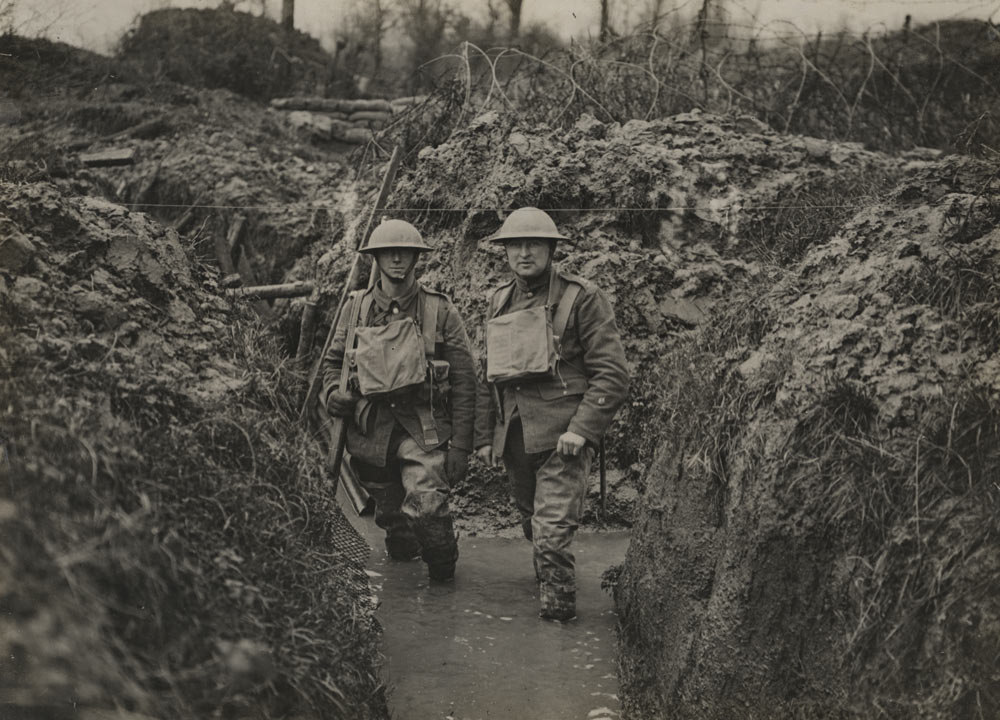
\includegraphics[keepaspectratio, height=\paperheight]{../img/wwi_trenches}};
  \end{tikzpicture}
\end{frame}
% ----------------------------------------------------
\note{Trincheras de la Primera Guerra Mundial. Más de 15 millones de muertos. Los líderes europeos creían que la guerra terminaría antes de Navidad; duró cuatro años. ¿Por qué no se evitó?}

% ----------------------------------------------------
\begin{frame}
\frametitle{La guerra como puzzle}
\centering

\begin{itemize}
  \item La guerra es \textbf{enormemente costosa}
  \begin{itemize}
    \item Vidas humanas, destrucción material, costes económicos
  \end{itemize}
  \item<2-> Si todos pierden con la guerra...
  \item<2-> ¿por qué no llegan a un acuerdo para evitarla?
  \vspace{8pt}
  \item<3-> Ésta es la pregunta central de este tema
\end{itemize}

\end{frame}
% ----------------------------------------------------
\note{Plantear el puzzle con claridad. No basta con decir ``tenían intereses enfrentados''. Las guerras entre Irak e Irán, la IIGM, la guerra de Irak de 2003 -- todas fueron desastrosas para al menos uno de los bandos, y a menudo para todos. Si hay un acuerdo que ambos prefieren a la guerra, ¿por qué no lo alcanzan?}


% ====================================================
\section{Intereses en conflicto}
% ====================================================

% ----------------------------------------------------
\begin{frame}
\frametitle{¿Por qué luchan los Estados?}
\centering

\begin{itemize}
  \item \textbf{Territorio:} recursos, posición estratégica, identidad
  \begin{itemize}
    \item Históricamente la causa más frecuente de guerra
  \end{itemize}
  \item<2-> \textbf{Políticas:} cuando un Estado adopta políticas que perjudican a otro
  \begin{itemize}
    \item Armas de destrucción masiva, derechos humanos
  \end{itemize}
  \item<3-> \textbf{Régimen:} la composición del gobierno de otro Estado
  \begin{itemize}
    \item Cambio de régimen, intervenciones durante la Guerra Fría
  \end{itemize}
\end{itemize}

\end{frame}
% ----------------------------------------------------
\note{Tres grandes categorías de conflictos de interés (FLS):
\begin{enumerate}
  \item Territorio: más de la mitad de las guerras en los últimos 300 años. Ejemplos: Irán-Irak (petróleo), Israel-Siria (Altos del Golán), India-Pakistán (Cachemira)
  \item Políticas: Irak y armas de destrucción masiva, Corea del Norte, Kosovo (EE.UU. bombardeó Serbia por la represión contra los kosovares)
  \item Régimen: la Guerra Fría está llena de ejemplos -- Vietnam, Guatemala, Chile
\end{enumerate}
Pero los intereses en conflicto son condición \textit{necesaria} pero no \textit{suficiente} para la guerra.}

% ----------------------------------------------------
\begin{frame}
\frametitle{¿Qué es una guerra?}
\centering

\begin{itemize}
  \item Uso \textbf{organizado} de la fuerza militar
  \item Al menos \textbf{dos} partes
  \item Umbral mínimo de severidad (1.000 muertes en combate)
  \item<2-> Tipos:
  \begin{itemize}
    \item \textbf{Guerra interestatal:} entre Estados
    \item \textbf{Guerra civil:} dentro de un Estado
  \end{itemize}
\end{itemize}

\end{frame}
% ----------------------------------------------------
\note{Definición técnica. El umbral de 1.000 muertes es el estándar del proyecto Correlates of War. Esto excluye escaramuzas menores, pero incluye conflictos como la guerra de las Malvinas (907 muertos, a veces incluida). Hoy nos centramos en guerras interestatales; las guerras civiles y el terrorismo los veremos en la sesión 5.}


% ====================================================
\section{El modelo de negociación}
% ====================================================

% ----------------------------------------------------
\begin{frame}
\frametitle{Una observación clave}
\centering

\begin{itemize}
  \item La mayoría de los conflictos entre Estados se resuelven \textbf{sin guerra}
  \item La guerra es la \textbf{excepción}, no la regla
  \item<2-> Entonces no basta con preguntar \textit{``¿por qué luchan?''}
  \item<2-> También hay que preguntar \textit{``¿por qué \textbf{no} llegan a un acuerdo?''}
\end{itemize}

\end{frame}
% ----------------------------------------------------
\note{Dato: en cualquier año dado, el porcentaje de Estados en guerra es muy bajo. Hay miles de disputas territoriales, políticas y de régimen que se resuelven sin violencia. La paz no se explica por falta de desacuerdos: hay conflictos de intereses todo el tiempo. Lo que necesitamos explicar es por qué \textit{a veces} falla la negociación.}

% ----------------------------------------------------
\begin{frame}
\frametitle{La negociación bajo amenaza de fuerza}
\centering

\begin{itemize}
  \item En ausencia de instituciones internacionales fuertes, los Estados resuelven sus conflictos mediante \textbf{negociación}
  \item<2-> Crisis: al menos un Estado amenaza con usar la fuerza
  \begin{itemize}
    \item ``Acepta mis demandas, o si no...''
  \end{itemize}
  \item<2-> Negociación coercitiva (\textit{crisis bargaining})
\end{itemize}

\end{frame}
% ----------------------------------------------------
\note{A diferencia de la política doméstica, no hay tribunales ni policía que resuelvan disputas entre Estados. Los conflictos se resuelven mediante negociación, donde la amenaza de fuerza es una herramienta. Ejemplo: ultimátum de Bush a Saddam Hussein (48 horas para irse de Irak) o la movilización rusa en la frontera de Ucrania en 2014. La negociación coercitiva es la ``diplomacia coercitiva'': combinar amenazas con ofertas.}

% ----------------------------------------------------
\begin{frame}
\frametitle{El rango de negociación}
\centering

\vspace{-5pt}
\begin{tikzpicture}[scale=0.85]
  % The bar
  \fill[accent!15] (0, 0) rectangle (10, 0.6);
  \draw[thick] (0, 0) rectangle (10, 0.6);

  % Labels
  \node[font=\footnotesize, anchor=south] at (0, 0.7) {Ideal A};
  \node[font=\footnotesize, anchor=south] at (10, 0.7) {Ideal B};

  % War outcome
  \draw[thick, accent2, dashed] (5.5, -0.2) -- (5.5, 0.8);
  \node[font=\scriptsize, accent2, anchor=south] at (5.5, 0.85) {Resultado esperado de la guerra};

  % Costs
  \draw[thick, accent, <->] (3.8, -0.5) -- (7.2, -0.5);
  \node[font=\scriptsize, accent, anchor=north] at (5.5, -0.55) {Rango de negociación};

  % Cost labels
  \draw[thick, accent!60] (3.8, -0.2) -- (3.8, 0.8);
  \node[font=\tiny, anchor=south east] at (3.7, 0.85) {Valor de guerra A};
  \draw[thick, accent!60] (7.2, -0.2) -- (7.2, 0.8);
  \node[font=\tiny, anchor=south west] at (7.3, 0.85) {Valor de guerra B};

  % Arrows for costs
  \draw[thick, red!60, <->] (3.8, -1.1) -- (5.5, -1.1);
  \node[font=\tiny, red!60!black] at (4.65, -1.4) {Costes de A};
  \draw[thick, red!60, <->] (5.5, -1.1) -- (7.2, -1.1);
  \node[font=\tiny, red!60!black] at (6.35, -1.4) {Costes de B};

\end{tikzpicture}

\vspace{8pt}
\begin{itemize}
  \item[\color{accent}$\bullet$] \footnotesize Los costes de la guerra crean un \textbf{rango de acuerdos} que ambos prefieren a la guerra
\end{itemize}

\end{frame}
% ----------------------------------------------------
\note{Diagrama central del capítulo. La barra representa el bien en disputa (territorio, por ejemplo). Cada Estado prefiere más para sí. Si van a la guerra, el resultado esperado está en algún punto de la barra, pero ambos pagan costes. Esos costes crean un rango de acuerdos que ambos prefieren a pelear.

Ejemplo numérico: territorio vale 100M. A espera ganar. Costes de guerra para A: 30M. Valor de guerra para A = 70M. A acepta cualquier acuerdo que le dé al menos 70M. Si los costes de B son 20M, B acepta cualquier acuerdo que le deje al menos lo equivalente a lo que ganaría en la guerra menos 20M. El rango de negociación es la zona donde ambos están satisfechos.

Implicación: \textbf{siempre} existe un rango de negociación si la guerra tiene costes para ambos.}

% ----------------------------------------------------
\begin{frame}
\frametitle{Ejemplo: el rango de negociación}
\centering

\footnotesize
\begin{itemize}
  \item A y B disputan un territorio valorado en \textbf{100 millones}
  \item A espera ganar la guerra; costes de A = 30M
  \item<2-> Valor de guerra para A = 100 $-$ 30 = \textbf{70M}
  \item<2-> A acepta cualquier acuerdo que le dé $\geq$ 70M
  \item<3-> B espera perder; costes de B = 20M
  \item<3-> Valor de guerra para B = 0 $-$ 20 = \textbf{$-$20M}
  \item<3-> B acepta cualquier acuerdo que le cueste $\leq$ 20M
  \item<4-> \textbf{Rango de negociación:} A recibe entre 70 y 80M
  \item<4-> Ambos prefieren \textit{cualquier} acuerdo en ese rango a la guerra
\end{itemize}

\end{frame}
% ----------------------------------------------------
\note{Ejemplo numérico concreto para fijar la intuición del diagrama anterior. El territorio vale 100M. A espera ganar, así que sin costes se quedaría con los 100M; pero la guerra le cuesta 30M, así que el valor de la guerra para A es 70M. Cualquier acuerdo que dé a A al menos 70M es mejor que luchar. Para B es simétrico: espera perder y además pagar 20M en costes. Acepta perder hasta 20M sin luchar. El rango donde ambos están de acuerdo es que A reciba entre 70M y 80M. Cuanto mayores los costes de guerra, más amplio es el rango de negociación.}

% ----------------------------------------------------
\begin{frame}
\centering
\vspace{30pt}

{\large ¿Se os ocurre un conflicto real en el que ambos bandos hubieran estado mejor con un acuerdo negociado?}

\vspace{15pt}
\footnotesize ¿Por qué no lo alcanzaron?

\end{frame}
% ----------------------------------------------------
\note{Pregunta de discusión para activar la participación. Respuestas posibles: IGM (todos perdieron), guerra de Irak 2003 (EE.UU. podría haber evitado una ocupación costosa), guerra Irán-Irak (8 años, más de un millón de muertos, ningún cambio territorial significativo). Usar las respuestas para conectar con las tres causas de fracaso que vamos a ver.}


% ====================================================
\section{Compelencia y disuasión}
% ====================================================

% ----------------------------------------------------
\begin{frame}
\frametitle{Compelencia y disuasión}
\centering

\begin{itemize}
  \item \textbf{Compelencia} (\textit{compellence}): amenazar con la fuerza para \textit{cambiar} el statu quo
  \begin{itemize}
    \item ``Dame \textit{x}, o si no...''
    \item ``Deja de hacer \textit{y}, o si no...''
  \end{itemize}
  \item<2-> \textbf{Disuasión} (\textit{deterrence}): amenazar con la fuerza para \textit{preservar} el statu quo
  \begin{itemize}
    \item ``No hagas \textit{x}, o si no...''
    \item General: ``no me ataques''
    \item Extendida: ``no ataques a mi aliado''
  \end{itemize}
\end{itemize}

\end{frame}
% ----------------------------------------------------
\note{Dos tipos de amenazas:
\begin{enumerate}
  \item Compelencia: EE.UU. exige a Afganistán que entregue a Bin Laden (2001). Irak exige a Kuwait que ceda territorio y condone deuda (1990)
  \item Disuasión general: todos los Estados la practican constantemente (``si me atacas, me defiendo''). Disuasión extendida: EE.UU. protege a Corea del Sur, la OTAN protege a sus miembros
\end{enumerate}
La disuasión extendida es más difícil de hacer creíble porque el que disuade no está directamente amenazado. La Guerra Fría giraba en torno a esto: ¿sacrificaría EE.UU. Nueva York para defender Londres o París?}


% ====================================================
\section{Información incompleta}
% ====================================================

% ----------------------------------------------------
\begin{frame}
\frametitle{¿Por qué falla la negociación? (I)}
\centering

{\Large \textbf{Información incompleta}}

\vspace{15pt}

\begin{itemize}
  \item Los Estados no saben con certeza cuánto puede y quiere luchar el adversario
  \item<2-> Dos incógnitas clave:
  \begin{itemize}
    \item \textbf{Capacidades:} tropas, armamento, tecnología, aliados
    \item \textbf{Determinación} (\textit{resolve}): disposición a asumir costes
  \end{itemize}
\end{itemize}

\end{frame}
% ----------------------------------------------------
\note{Primera causa de fracaso en la negociación. La analogía del póker es útil: cada jugador conoce sus propias cartas pero no las del adversario. Información privada.

Capacidades: son parcialmente observables (satélites, informes de inteligencia) pero no del todo. Ejemplo: el plan del ``gancho izquierdo'' de EE.UU. en 1991 (flanqueo por el desierto en vez de ataque frontal en Kuwait).

Determinación: aún más difícil de medir. ¿Cuántas vidas está dispuesto a sacrificar un país por un territorio? Depende de factores políticos, ideológicos, psicológicos. Ejemplo: Saddam Hussein creía que EE.UU. ``no podría aceptar 10.000 muertos en una batalla''. Se equivocó.}

% ----------------------------------------------------
\begin{frame}
\frametitle{El trade-off riesgo-beneficio}
\centering

\begin{itemize}
  \item Cuando hay incertidumbre, cada Estado enfrenta un dilema:
  \item<2-> Ceder mucho $\rightarrow$ paz segura, pero mal acuerdo
  \item<2-> No ceder $\rightarrow$ mejor acuerdo si funciona, pero riesgo de guerra
  \vspace{8pt}
  \item<3-> Este \textbf{trade-off entre riesgo y beneficio} puede llevar racionalmente a la guerra
\end{itemize}

\end{frame}
% ----------------------------------------------------
\note{El trade-off riesgo-beneficio (risk-return trade-off). Kuwait en 1990: podría haber cedido a todas las demandas de Irak y evitado la guerra. Pero no quería ``paz a cualquier precio''. Kuwait eligió una estrategia que ofrecía un mejor resultado (no ceder) pero con mayor riesgo (invasión). No fue irracional: era una apuesta razonable dada la incertidumbre sobre las intenciones de Saddam.

Insight clave: la guerra puede ocurrir aunque ambos bandos sean racionales, simplemente porque no tienen suficiente información sobre el otro.}

% ----------------------------------------------------
\begin{frame}
\frametitle{El problema de la credibilidad}
\centering

\begin{itemize}
  \item ¿Por qué no se comunican la información?
  \item<2-> Porque los Estados tienen incentivos para \textbf{mentir o exagerar}
  \begin{itemize}
    \item Ocultar debilidades (parecer más fuerte)
    \item Farolear (\textit{bluff}): amenazar sin intención de cumplir
  \end{itemize}
  \item<3-> Un mensaje solo es útil si es \textbf{creíble}
  \begin{itemize}
    \item ¿Me creerá el adversario?
  \end{itemize}
\end{itemize}

\end{frame}
% ----------------------------------------------------
\note{Problema central de la comunicación estratégica. Ejemplo histórico:
\begin{itemize}
  \item China en Corea (1950): advirtió a EE.UU. a través del embajador indio que intervendría si EE.UU. cruzaba el paralelo 38. Dean Acheson lo descartó como un farol porque el mensaje era ``barato'' -- no le costaba nada a China enviarlo. Resultado: EE.UU. cruzó y 600.000 soldados chinos entraron en la guerra
  \item Hitler y Renania (1936): envió tropas a la zona desmilitarizada. Francia y Gran Bretaña no reaccionaron. Hay evidencia de que era un farol: las tropas tenían órdenes de retirarse si les plantaban cara
\end{itemize}
El dilema: ¿cómo enviar una señal creíble de que NO estás faroleando?}


% ====================================================
\section{Señales costosas}
% ====================================================

% ----------------------------------------------------
\begin{frame}
\frametitle{¿Cómo hacer creíbles las amenazas?}
\centering

\begin{itemize}
  \item Para ser creíble, una amenaza debe ser \textbf{costosa} de hacer
  \item<2-> Tres mecanismos:
  \begin{enumerate}
    \item<2-> \textbf{Brinksmanship} (diplomacia al borde del abismo)
    \item<3-> \textbf{Atarse las manos} (\textit{tying hands})
    \item<4-> \textbf{Pagar para tener poder} (\textit{paying for power})
  \end{enumerate}
\end{itemize}

\end{frame}
% ----------------------------------------------------
\note{Idea general (Schelling): las amenazas baratas no son creíbles. Para demostrar que hablas en serio, tienes que hacer algo que te cueste -- algo que no harías si estuvieras faroleando. Tres estrategias concretas que vamos a ver.}

% ----------------------------------------------------
\begin{frame}
\frametitle{Brinksmanship}
\centering

\begin{itemize}
  \item Aumentar deliberadamente el riesgo de que la guerra estalle \textit{por accidente}
  \item ``El borde del precipicio no es un acantilado donde uno se para y decide si salta; es una pendiente resbaladiza'' (Schelling)
  \item<2-> Cada bando sube la apuesta hasta que uno cede... o caen juntos
\end{itemize}

\end{frame}
% ----------------------------------------------------
\note{Concepto de Thomas Schelling (Premio Nobel). No es una amenaza de empezar una guerra deliberadamente -- eso no sería creíble si la guerra es catastrófica (especialmente nuclear). Es crear una situación donde la guerra puede empezar por accidente o escalada.

Ejemplo paradigmático: la crisis de los misiles de Cuba (1962). Kennedy y Jrushchov no querían una guerra nuclear, pero ambos tomaron medidas (bloqueo naval, bases de misiles) que aumentaban el riesgo de un incidente que desencadenara la escalada. Un incidente real: un U-2 americano fue derribado sobre Cuba. La tensión era tal que cualquier error podía ser el último.

La disposición a asumir ese riesgo separa a los que van en serio de los que farolean.}

% ----------------------------------------------------
\begin{frame}[plain]
  \begin{tikzpicture}[remember picture, overlay]
    \node[at = (current page.center), yshift = 0cm] (cover) {%
      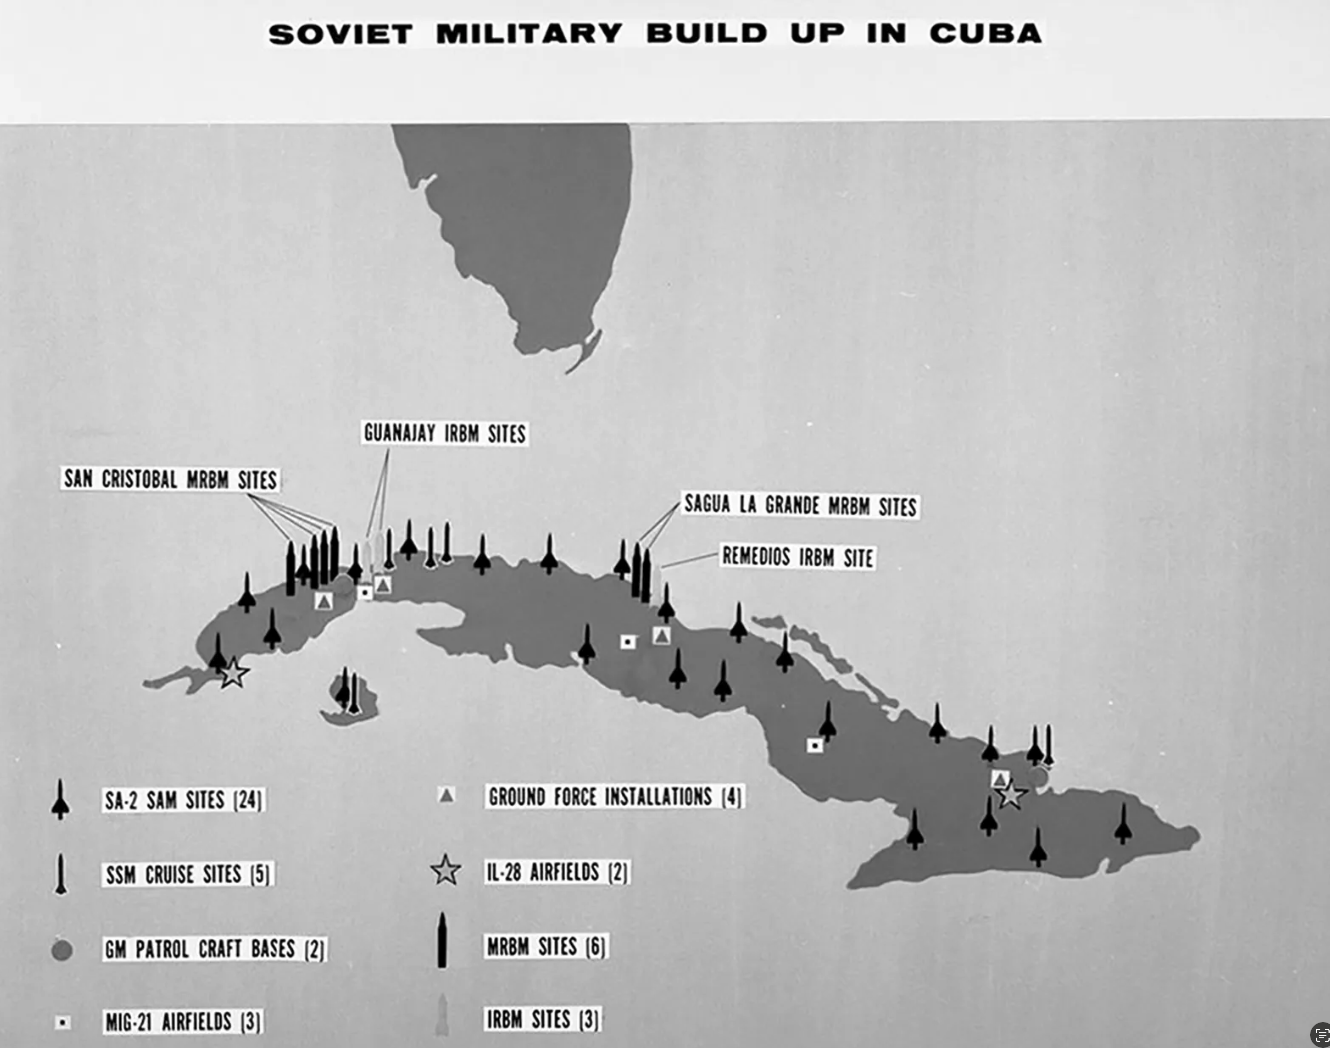
\includegraphics[keepaspectratio, height=\paperheight]{../img/cuban_missile_crisis}};
  \end{tikzpicture}
\end{frame}
% ----------------------------------------------------
\note{Crisis de los misiles de Cuba (1962). Ejemplo clásico de brinksmanship. Kennedy impuso un bloqueo naval a Cuba; Jrushchov tenía barcos soviéticos acercándose. Ambos bandos sabían que un choque naval podía escalar a guerra nuclear. Al final, Jrushchov retiró los misiles a cambio de la promesa de EE.UU. de no invadir Cuba (y la retirada secreta de misiles americanos de Turquía).}

% ----------------------------------------------------
\begin{frame}
\frametitle{Atarse las manos}
\centering

\begin{itemize}
  \item Hacer declaraciones públicas o tomar acciones de las que sea difícil echarse atrás
  \item<2-> Si el líder no cumple su amenaza, paga \textbf{costes de audiencia}
  \begin{itemize}
    \item Reputación internacional dañada
    \item Castigo electoral doméstico
  \end{itemize}
  \item<2-> Ejemplo: Bush tras la invasión de Kuwait: ``This will not stand''
\end{itemize}

\end{frame}
% ----------------------------------------------------
\note{Costes de audiencia (audience costs). Cuando un líder hace una declaración pública, se juega su reputación. Retirarse después es humillante y puede costar votos.

Ejemplo positivo: Bush en 1990 -- desplegó 500.000 tropas y declaró públicamente que la invasión de Kuwait no sería aceptada. Retroceder habría sido devastador políticamente.

Ejemplo de fracaso: Obama y la ``línea roja'' en Siria (2012). Dijo que el uso de armas químicas tendría consecuencias. Cuando Siria las usó, Obama no atacó. Fue muy criticado por haber hecho una amenaza vacía.

La idea: atarse las manos envía un mensaje poderoso: ``No puedo retirarme; mi amenaza es totalmente creíble.''}

% ----------------------------------------------------
\begin{frame}
\frametitle{Pagar para tener poder}
\centering

\begin{itemize}
  \item Tomar medidas costosas para aumentar las capacidades militares
  \begin{itemize}
    \item Movilización de tropas, aumento del gasto militar
  \end{itemize}
  \item<2-> Dos efectos:
  \begin{itemize}
    \item Reduce el coste de cumplir la amenaza
    \item Señala que el Estado se toma en serio la disputa
  \end{itemize}
  \item<2-> Ejemplo: Kennedy aumentó el ejército en 350.000 soldados durante la crisis de Berlín (1961)
\end{itemize}

\end{frame}
% ----------------------------------------------------
\note{Tercer mecanismo. Las movilizaciones militares no solo son preparativos para la guerra: también son señales. Si un Estado gasta grandes cantidades de dinero y recursos, demuestra que le importa lo suficiente como para luchar. Kennedy llamó a reservistas -- personas que ya habían terminado su servicio militar y tenían familias y trabajos. Eso es políticamente costoso, lo que hace la señal más creíble.

Pero ojo: estos tres mecanismos son ``curas'' para la información incompleta que pueden ser tan peligrosas como la enfermedad. El brinksmanship crea riesgo de accidente; atarse las manos puede llevar a posiciones irreconciliables; las movilizaciones pueden provocar al adversario a atacar primero.}


% ====================================================
\section{Problemas de compromiso}
% ====================================================

% ----------------------------------------------------
\begin{frame}
\frametitle{¿Por qué falla la negociación? (II)}
\centering

{\Large \textbf{Problemas de compromiso}}

\vspace{15pt}

\begin{itemize}
  \item A veces el acuerdo pacífico existe, pero...
  \item<2-> ¿Puedo confiar en que el adversario \textbf{cumplirá} el acuerdo en el futuro?
  \item<3-> Si no hay forma de garantizarlo, puede ser mejor luchar \textit{ahora}
\end{itemize}

\end{frame}
% ----------------------------------------------------
\note{Segunda gran categoría de causas de la guerra. Incluso si ambos Estados saben cuáles son las capacidades y la determinación del otro, puede haber guerra si uno no puede comprometerse creíblemente a respetar el acuerdo.

A nivel doméstico, los tribunales y la policía hacen cumplir los contratos. A nivel internacional, no hay equivalente. Tres variantes de este problema.}

% ----------------------------------------------------
\begin{frame}
\frametitle{Bienes que dan poder}
\centering

\begin{itemize}
  \item Cuando el bien en disputa es fuente de \textbf{poder futuro}
  \begin{itemize}
    \item Territorio estratégico, armas nucleares
  \end{itemize}
  \item<2-> Ceder hoy $\rightarrow$ el adversario se fortalece $\rightarrow$ mañana exige más
  \item<2-> Ejemplo: Libia (2003) abandonó su programa nuclear a cambio de promesas... en 2011 fue intervenida
\end{itemize}

\end{frame}
% ----------------------------------------------------
\note{El caso de Libia es muy instructivo. Gadafi renunció a sus armas químicas y nucleares en 2003 a cambio de normalización con EE.UU. y UK. En 2011, cuando estalló una rebelión, EE.UU. y UK intervinieron militarmente y Gadafi fue derrocado y asesinado. La lección (para Corea del Norte, Irán): una promesa de no atacar no es necesariamente creíble ni duradera.

Otro ejemplo: China y Japón disputan las islas Senkaku/Diaoyu en el Mar de China Oriental. El control de las islas afecta al equilibrio militar regional.

Si ceder un bien te hace más vulnerable y no hay forma de garantizar que el adversario no lo explotará, puede ser racional preferir la guerra.}

% ----------------------------------------------------
\begin{frame}
\frametitle{Guerra preventiva}
\centering

\begin{itemize}
  \item Cuando el equilibrio de poder está cambiando
  \begin{itemize}
    \item Crecimiento económico desigual, nuevas tecnologías
  \end{itemize}
  \item<2-> El Estado que se debilita puede preferir luchar \textbf{hoy} antes de que sea más débil \textbf{mañana}
  \item<2-> No puede confiar en que el Estado creciente no explotará su ventaja futura
\end{itemize}

\end{frame}
% ----------------------------------------------------
\note{Guerra preventiva: luchar ahora para impedir que el adversario se fortalezca. El Estado creciente no puede comprometerse creíblemente a no usar su futuro poder.

Ejemplo histórico: Alemania en 1914. Los líderes alemanes veían con preocupación el crecimiento económico e industrial de Rusia. Creían que tenían una ``ventana de oportunidad'' cada vez más estrecha. Mejor luchar en 1914 que en 1920, cuando Rusia sería más fuerte.

Ejemplo contemporáneo: la invasión de Irak en 2003 tenía una lógica preventiva. El argumento era que sería más fácil derrocar a Saddam antes de que desarrollara armas de destrucción masiva que después.

Pregunta para los estudiantes: ¿tiene la competición entre EE.UU. y China elementos de lógica preventiva?}

% ----------------------------------------------------
\begin{frame}
\frametitle{Guerra preventiva: la Primera Guerra Mundial}
\centering

\vspace{-3pt}
\begin{tikzpicture}[scale=0.75]

  % Period bands
  \fill[accent!10] (0, -0.15) rectangle (5, -0.55);
  \fill[red!12] (5, -0.15) rectangle (10, -0.55);

  % Period labels
  \node[font=\tiny\itshape, accent!80!black] at (2.5, -0.35) {Crecimiento ruso};
  \node[font=\tiny\itshape, red!60!black] at (7.5, -0.35) {``Ventana de oportunidad'' alemana se cierra};

  % Main timeline
  \draw[thick, jet!50, ->] (-0.3, 0) -- (10.5, 0);

  % 1890 - growing Russian economy
  \fill[jet] (1, 0) circle (2pt);
  \draw[jet!30] (1, 0) -- (1, 1.5);
  \node[font=\tiny, align=center, anchor=south] at (1, 1.55) {%
    \textbf{$\sim$1890}\\Industrialización\\rusa};

  % 1905
  \fill[jet] (3.5, 0) circle (2pt);
  \draw[jet!30] (3.5, 0) -- (3.5, 0.8);
  \node[font=\tiny, align=center, anchor=south] at (3.5, 0.85) {%
    \textbf{1905}\\Derrota rusa\\vs.~Japón};

  % 1907
  \fill[jet] (5, 0) circle (2pt);
  \draw[jet!30] (5, 0) -- (5, 1.5);
  \node[font=\tiny, align=center, anchor=south] at (5, 1.55) {%
    \textbf{1907}\\Triple\\Entente};

  % June 1914
  \fill[jet] (7.5, 0) circle (2pt);
  \draw[jet!30] (7.5, 0) -- (7.5, 0.8);
  \node[font=\tiny, align=center, anchor=south] at (7.5, 0.85) {%
    \textbf{Jun 1914}\\Asesinato del\\Archiduque};

  % August 1914
  \fill[accent2] (9.5, 0) circle (3pt);
  \draw[accent2!50] (9.5, 0) -- (9.5, 1.5);
  \node[font=\tiny, align=center, anchor=south, accent2] at (9.5, 1.55) {%
    \textbf{Ago 1914}\\Estalla\\la IGM};

\end{tikzpicture}

\vspace{8pt}
\footnotesize
\begin{itemize}
  \item Alemania temía el crecimiento de Rusia
  \item El Plan Schlieffen dependía de atacar primero
  \item Incentivos preventivos + preemptivos
\end{itemize}

\end{frame}
% ----------------------------------------------------
\note{La IGM combina prevención y preemptividad:
\begin{enumerate}
  \item Prevención: Alemania veía crecer a Rusia y creía que en pocos años sería imparable. Mejor luchar ahora
  \item Preemptividad: el Plan Schlieffen buscaba explotar la lentitud de la movilización rusa para derrotar primero a Francia. Había una ventaja enorme para quien atacase primero
  \item Cuando Rusia movilizó el 30 de julio de 1914 como señal de determinación (para disuadir a Austria), provocó exactamente lo contrario: Alemania activó el Plan Schlieffen. El 3 de agosto, Europa estaba en guerra
\end{enumerate}
Lección: las movilizaciones, que en teoría son señales de determinación, pueden provocar guerra cuando hay incentivos preemptivos.}

% ----------------------------------------------------
\begin{frame}
\frametitle{Guerra preemptiva}
\centering

\begin{itemize}
  \item Cuando hay una \textbf{ventaja de primer golpe}
  \begin{itemize}
    \item La tecnología o la estrategia militar favorecen al que ataca primero
  \end{itemize}
  \item<2-> Si ninguno puede comprometerse a no atacar, ambos tienen incentivos para adelantarse
  \item<2-> Ejemplo: Israel en 1967 -- destruyó la fuerza aérea egipcia en tierra
\end{itemize}

\end{frame}
% ----------------------------------------------------
\note{Guerra de los Seis Días (1967): tras semanas de tensión y movilización egipcia, Israel lanzó un ataque sorpresa y destruyó 300 aviones egipcios en tierra. Había una ventaja enorme de primer golpe: si Israel esperaba, Egipto podía atacar primero.

El dilema de seguridad se agrava cuando la tecnología favorece la ofensiva: armarse para defenderse hace que el otro sienta que le vas a atacar, lo cual le lleva a armarse, lo cual te hace sentir más amenazado...

Diferencia entre prevención y preemptividad:
\begin{itemize}
  \item Prevención = respuesta a cambios en el equilibrio de poder a largo plazo
  \item Preemptividad = respuesta a una amenaza inminente con ventaja de primer golpe
\end{itemize}}

% ----------------------------------------------------
\begin{frame}
\frametitle{Preventiva vs. preemptiva}
\centering

\vspace{5pt}
\begin{columns}[T]
\begin{column}{0.45\textwidth}
\centering
\textbf{Guerra preventiva}

\vspace{8pt}
\footnotesize
\begin{itemize}
  \item Cambios en el equilibrio de poder \textbf{a largo plazo}
  \item Luchar \textit{ahora} antes de debilitarse
  \item Ej: Alemania vs. Rusia (1914)
  \item Ej: EE.UU. vs. Irak (2003)
\end{itemize}
\end{column}
\begin{column}{0.45\textwidth}
\centering
\textbf{Guerra preemptiva}

\vspace{8pt}
\footnotesize
\begin{itemize}
  \item Amenaza \textbf{inminente} + ventaja de primer golpe
  \item Atacar antes de que el otro ataque
  \item Ej: Israel vs. Egipto (1967)
  \item Ej: Plan Schlieffen (1914)
\end{itemize}
\end{column}
\end{columns}

\vspace{10pt}
\footnotesize
Ambas son \textbf{problemas de compromiso}: no se puede confiar en que el otro no explotará su ventaja.

\end{frame}
% ----------------------------------------------------
\note{Slide de comparación directa. Ambas son variantes del problema de compromiso, pero operan en escalas temporales distintas. La preventiva responde a tendencias de largo plazo (crecimiento económico, desarrollo tecnológico); la preemptiva a una amenaza inmediata donde horas o días importan. La IGM combina ambas lógicas: Alemania tenía motivaciones preventivas frente a Rusia Y preemptivas por el Plan Schlieffen.}

% ----------------------------------------------------
\begin{frame}
\centering
\vspace{30pt}

{\large ¿Tiene la competición entre EE.UU. y China elementos de lógica preventiva?}

\vspace{15pt}
\footnotesize ¿Y qué mecanismos podrían reducir ese riesgo?

\end{frame}
% ----------------------------------------------------
\note{Segunda pregunta de discusión. China es la potencia en ascenso; EE.UU. la potencia establecida. Algunos analistas hablan de ``la trampa de Tucídides'' (Allison). Respuestas posibles sobre mecanismos: interdependencia económica (mayor que antes de la IGM), armas nucleares (disuasión mutua), instituciones internacionales (G20, ONU). Conectar con la sección final sobre el declive de la guerra interestatal.}


% ====================================================
\section{Bienes indivisibles}
% ====================================================

% ----------------------------------------------------
\begin{frame}
\frametitle{¿Por qué falla la negociación? (III)}
\centering

{\Large \textbf{Bienes indivisibles}}

\vspace{15pt}

\begin{itemize}
  \item Algunos bienes no se pueden dividir sin perder su valor
  \item<2-> Si no hay forma de ``partir la diferencia'', la negociación puede fracasar
  \item<2-> No es una propiedad física sino de \textit{cómo se valora} el bien
\end{itemize}

\end{frame}
% ----------------------------------------------------
\note{Tercera causa. Recordar que el modelo de negociación asume que podemos dividir el bien. Pero ¿qué pasa si no se puede?

Ejemplo paradigmático: Jerusalén. Lugar sagrado para judaísmo, cristianismo e islam. Los sitios más sagrados de ambas religiones están literalmente uno encima del otro (el Muro de las Lamentaciones y la Explanada de las Mezquitas / Cúpula de la Roca). No se puede ``partir'' sin destruir su valor simbólico y religioso.

Pero cuidado: la indivisibilidad puede ser exagerada estratégicamente. Un gobierno puede declarar que ``Jerusalén no se negocia'' para atarse las manos. Además, hay mecanismos como el control compartido o la compensación en otro ámbito (\textit{linkage}) que pueden superar la indivisibilidad aparente.}


% ====================================================
\section{¿Se ha vuelto la guerra obsoleta?}
% ====================================================

% ----------------------------------------------------
\begin{frame}[plain]
  \begin{tikzpicture}[remember picture, overlay]
    \node[at = (current page.center), yshift = 0cm] (cover) {%
      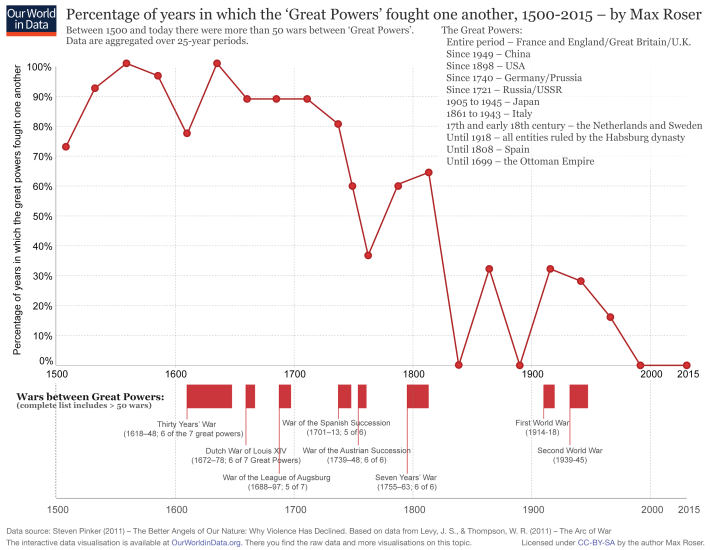
\includegraphics[keepaspectratio, height=\paperheight]{../img/great_powers_wars}};
  \end{tikzpicture}
\end{frame}
% ----------------------------------------------------
\note{Gráfico que muestra la frecuencia de guerras interestatales a lo largo del tiempo. Desde 1950, las guerras interestatales han disminuido notablemente. No ha habido guerra entre grandes potencias desde la guerra de Corea (1953). ¿Se está volviendo la guerra obsoleta?}

% ----------------------------------------------------
\begin{frame}
\frametitle{¿Por qué menos guerras? (Aplicando el marco I-I-I)}
\centering

\begin{itemize}
  \item \textbf{Intereses:} el territorio ha perdido importancia relativa
  \begin{itemize}
    \item Comercio y mercados vs. conquista
  \end{itemize}
  \item<2-> \textbf{Costes:} armas nucleares e interdependencia económica
  \begin{itemize}
    \item Destrucción mutua asegurada; costes comerciales de la guerra
  \end{itemize}
  \item<3-> \textbf{Instituciones:} democracia y organizaciones internacionales
  \begin{itemize}
    \item Paz democrática, verificación, mediación
  \end{itemize}
\end{itemize}

\end{frame}
% ----------------------------------------------------
\note{Aquí cerramos el tema aplicando explícitamente el marco I-I-I (Intereses, Interacciones, Instituciones) de la sesión anterior. Los tres factores corresponden directamente a cada dimensión del marco:
\begin{enumerate}
  \item Intereses: el nacionalismo ha hecho más costoso controlar poblaciones extranjeras; el comercio ha hecho más fácil acceder a recursos sin conquistar. EE.UU. impulsó la norma de ``integridad territorial'' después de 1945
  \item Costes: las armas nucleares han hecho la guerra entre grandes potencias potencialmente suicida. La interdependencia económica (comercio, finanzas) ha aumentado los costes
  \item Instituciones: la democracia y las organizaciones internacionales (OIEA, ONU, OMC) han mejorado la información y facilitado los compromisos
\end{enumerate}
Pero ojo: ¿significa esto que la guerra ha desaparecido? Ucrania, Gaza... La próxima semana veremos más sobre política doméstica y organizaciones internacionales.}


% ====================================================

% ----------------------------------------------------
\begin{frame}
\frametitle{Resumen}
\centering

\begin{itemize}
  \item La guerra es \textbf{costosa} $\rightarrow$ siempre existe un rango de negociación
  \item Pero la negociación puede fallar por:
  \begin{enumerate}
    \item \textbf{Información incompleta} sobre capacidades y determinación
    \item \textbf{Problemas de compromiso} (bienes que dan poder, prevención, preemptividad)
    \item \textbf{Bienes indivisibles} ligados a valores fundamentales
  \end{enumerate}
  \item<2-> Factores que reducen la guerra: menor valor del territorio, armas nucleares, interdependencia económica, democracia, organizaciones internacionales
\end{itemize}

\end{frame}
% ----------------------------------------------------
\note{Recapitulación. La clave es que la guerra no se explica solo por intereses en conflicto (los hay todo el tiempo). Se explica por el fracaso de la negociación debido a estos tres tipos de problemas. La próxima semana: ¿cómo influyen la política doméstica y las organizaciones internacionales en la probabilidad de guerra?}

% ----------------------------------------------------
\begin{frame}
\frametitle{}
\centering

Preguntas?

\end{frame}
% ----------------------------------------------------
\note{}
